%% (Master) Thesis template
% Template version used: v1.4
%
% Largely adapted from Adrian Nievergelt's template for the ADPS
% (lecture notes) project.


%% We use the memoir class because it offers a many easy to use features.
\documentclass[11pt,a4paper,oneside]{memoir}

%% Packages
%% ========

%% LaTeX Font encoding and language
\usepackage[T1]{fontenc}
\usepackage[utf8]{inputenc}
\usepackage[english]{babel}

% Use Latin Modern (a standard, CM-like font family commonly used for
% academic papers). Computer Modern math will be used (good default math
% appearance for papers).
\usepackage{lmodern}
\usepackage{microtype}

%% [REC] TikZ is used to draw figures
\usepackage{tikz}
% For positioning library (helps position nodes more easily), 
% and arrows.meta for more arrow tips and styles
\usetikzlibrary{
  decorations.pathreplacing,
  calc,
  shapes,
  arrows.meta,
  positioning,
  backgrounds,
  fit,
  matrix,
  graphs,
  graphs.standard, 
  positioning, 
  arrows.meta,
  patterns,
  shapes.geometric,
  shapes.misc,
  decorations.pathmorphing,
  shadows,
}



%% The AMS-LaTeX extensions for mathematical typesetting.  Do not
%% remove.  
\usepackage{amsmath,amsfonts,mathrsfs}


%% NTheorem is a reimplementation of the AMS Theorem package. This
%% will allow us to typeset theorems like examples, proofs and
%% similar.  Do not remove.
%% NOTE: Must be loaded AFTER amsmath, or the \qed placement will
%% break
\usepackage[amsmath,thmmarks]{ntheorem}
 
%% LaTeX' own graphics handling
\usepackage{graphicx}

% Search for graphics in the `logos/` subdirectory as well
\graphicspath{{logos/}}

%% We unfortunately need this for the Rules chapter.  Remove it
%% afterwards; or at least NEVER use its underlining features.
\usepackage{soul} 

%% This allows you to add .pdf files. It is used to add the
%% declaration of originality.
\usepackage{pdfpages}

%% Some more packages that you may want to use.  Have a look at the
%% file, and consult the package docs for each.
\input{thesis_settings/extrapackages.tex}

%% Our layout configuration.  DO NOT CHANGE.
%% Memoir layout setup

%% NOTE: You are strongly advised not to change any of them unless you
%% know what you are doing.  These settings strongly interact in the
%% final look of the document.

% Dependencies (logo packages in logos/)
\usepackage{logos/ETHlogo}
\usepackage{logos/UZHlogo}
\usepackage{logos/NYUlogo}

% --- Page geometry (memoir) - set smaller margins ---
% Set stock/trim sizes for A4 (height x width)
\setstocksize{297mm}{210mm}
\settrimmedsize{297mm}{210mm}{*}
% Set typeblock and margins: smaller margins (20mm on each side)
\settypeblocksize{*}{\dimexpr210mm-40mm\relax}{*}
\setlrmarginsandblock{27mm}{27mm}{*}% left/right margins
\setulmarginsandblock{27mm}{27mm}{*}% upper/lower margins
% apply
\checkandfixthelayout

% Turn extra space before chapter headings off.
\setlength{\beforechapskip}{0pt}

\nonzeroparskip
\parindent=0pt
\defaultlists

% Chapter style redefinition
\makeatletter

\if@twoside
  \pagestyle{Ruled}
  \copypagestyle{chapter}{Ruled}
\else
  \pagestyle{ruled}
  \copypagestyle{chapter}{ruled}
\fi
\makeoddhead{chapter}{}{}{}
\makeevenhead{chapter}{}{}{}
\makeheadrule{chapter}{\textwidth}{0pt}
\copypagestyle{abstract}{empty}

\makechapterstyle{bianchimod}{%
  \chapterstyle{default}
  \renewcommand*{\chapnamefont}{\normalfont\Large\rmfamily}
  \renewcommand*{\chapnumfont}{\normalfont\Large\rmfamily}
  \renewcommand*{\printchaptername}{%
    \chapnamefont\centering\@chapapp}
  \renewcommand*{\printchapternum}{\chapnumfont {\thechapter}}
  \renewcommand*{\chaptitlefont}{\normalfont\huge\rmfamily}
  \renewcommand*{\printchaptertitle}[1]{%
    \hrule\vskip\onelineskip \centering \chaptitlefont\textbf{\vphantom{gyM}##1}\par}
  \renewcommand*{\afterchaptertitle}{\vskip\onelineskip \hrule\vskip
    \afterchapskip}
  \renewcommand*{\printchapternonum}{%
    \vphantom{\chapnumfont {9}}\afterchapternum}}

% Use the newly defined style
\chapterstyle{bianchimod}

\setsecheadstyle{\Large\bfseries\rmfamily}
\setsubsecheadstyle{\large\bfseries\rmfamily}
\setsubsubsecheadstyle{\bfseries\rmfamily}
\setparaheadstyle{\normalsize\bfseries\rmfamily}
\setsubparaheadstyle{\normalsize\itshape\rmfamily}
\setsubparaindent{0pt}

% Set captions to a more separated style for clearness
\captionnamefont{\sffamily\bfseries\footnotesize}
\captiontitlefont{\sffamily\footnotesize}
\setlength{\intextsep}{16pt}
\setlength{\belowcaptionskip}{1pt}

% Set section and TOC numbering depth to subsection
\setsecnumdepth{subsection}
\settocdepth{subsection}

%% Titlepage adjustments
\pretitle{\vspace{0pt plus 0.7fill}\begin{center}\HUGE\rmfamily\bfseries}
\posttitle{\end{center}\par}
\preauthor{\par\begin{center}\let\and\\\Large\rmfamily}
\postauthor{\end{center}}
\predate{\par\begin{center}\Large\rmfamily}
\postdate{\end{center}}

\def\@advisors{}
\newcommand{\advisors}[1]{\def\@advisors{#1}}
\def\@department{} 
\newcommand{\department}[1]{\def\@department{#1}}
\def\@thesistype{}
\newcommand{\thesistype}[1]{\def\@thesistype{#1}}

% Show ETH logo on the left and UZH logo on the right in the title header
\renewcommand{\maketitlehooka}{%
  \noindent
  % Left logo in a top-aligned minipage exactly 2in wide
  \begin{minipage}[t]{2in}
    \UZHlogo[2in]%
  \end{minipage}%
  \hfill
  % Right logo in a top-aligned minipage exactly 2in wide
  \begin{minipage}[t]{2in}
    \raggedleft
    \ETHlogo[2in]%
  \end{minipage}%
}

\renewcommand{\maketitlehookb}{\vspace{1in}%
  \par\begin{center}\Large\rmfamily\@thesistype\end{center}}

\renewcommand{\maketitlehookd}{%
  \vfill\par
  \begin{flushright}
  \rmfamily
    \@advisors\par
    \@department, ETH Z\"urich
  \end{flushright}
}

\checkandfixthelayout

\setlength{\droptitle}{-48pt}

\makeatother

% This defines how theorems should look. Best leave as is.
\theoremstyle{plain}
\setlength\theorempostskipamount{0pt}

%%% Local Variables:
%%% mode: latex
%%% TeX-master: "thesis"
%%% End:


%% Theorem environments.  You will have to adapt this for a German
%% thesis.
\input{thesis_settings/theoremsetup.tex}

%% Helpful macros.
\input{thesis_settings/macrosetup.tex}

%% Make document internal hyperlinks wherever possible. (TOC, references)
\usepackage[linkcolor=black,colorlinks=true,citecolor=black,filecolor=black]{hyperref}

% Load cleveref after hyperref
\usepackage{cleveref}

% We now name most things that are to be referred to.
% You can add similar commands for your own defined environments
% THEOREM
\crefname{theorem}{theorem}{theorems}
\Crefname{theorem}{Theorem}{Theorems}

% LEMMA
\crefname{lemma}{lemma}{lemmas} 
\Crefname{lemma}{Lemma}{Lemmas}

% COROLLARY
\crefname{corollary}{corollary}{corollaries}
\Crefname{corollary}{Corollary}{Corollaries}

% PROPOSITION
\crefname{proposition}{proposition}{propositions}
\Crefname{proposition}{Proposition}{Propositions}

% CLAIM
\crefname{claim}{claim}{claims}
\Crefname{claim}{Claim}{Claims}

% DEFINITION
\crefname{definition}{definition}{definitions}
\Crefname{definition}{Definition}{Definitions}
% EXAMPLE
\crefname{example}{example}{examples}
\Crefname{example}{Example}{Examples}
%% The AMS-LaTeX extensions for mathematical typesetting.  Do not
%% remove. We avoid loading amssymb directly because `newtxmath` will
%% provide compatible symbol definitions; this prevents a \Bbbk clash.
\usepackage{amsmath,amsfonts,mathrsfs}
% REMARK
\crefname{remark}{remark}{remarks}
\Crefname{remark}{Remark}{Remarks}

% RULE - This one is special
\crefname{Rule}{rule}{rules}
\Crefname{Rule}{Rule}{Rules}

 
%% [REC] This is for restating theorems.
\usepackage{thmtools}
\usepackage{thm-restate}      


%% [REC] packages for pseudocode
\usepackage{algorithm}        % A float wrapper for algorithms
\usepackage{algorithmicx}
\usepackage{algpseudocode}


%% Document information
\title{Multi-Currency Portfolio Optimization with General Risk
Measures} 
\author{Anej Rozman}
\thesistype{Master Thesis} 
\advisors{Supervisor: Prof.\ Patrick Cheridito \\ Co-Supervisor: Dr.\ Urban Ulrych} 
\department{Department of Mathematics}   
\date{} 


%% ======================================================= %%
\begin{document}

\frontmatter  

%% Title page 
\begin{titlingpage} 
  \calccentering{\unitlength}
  \begin{adjustwidth*}{\unitlength-24pt}{-\unitlength-24pt}  
    \maketitle
  \end{adjustwidth*}
\end{titlingpage}

%% Acknowledgments
\chapter*{Acknowledgments}

% I would like to express my sincere gratitude to my supervisor, Prof.\ Patrick 
% Cheridito, for his guidance and support throughout the course of this thesis. 

% I would also like to thank my co-supervisor, Dr.\ Urban Ulrych, for his involvement and guidance on 
% the project. Throughtout the thesis. 

% Finally, I would like to thank my family and friends for their encouragement and support during this journey.
\pagebreak

%% Abstract 
\input{chapters/abstract.tex}  

%% TOC with the proper setup
\cleartorecto 
\tableofcontents
\mainmatter

%% Content
\newpage
\input{chapters/student_intro.tex}
\chapter{Literature Review}

In this chapter, we review the relevant literature on multi-currency 
portfolio optimization. We discuss the contributions and 
methodologies in the field, highlighting how our work builds 
upon and extends existing research. 

The core of our analysis builds on two recent studies that 
apply regularization techniques to international asset allocation. 
Burkhardt and Ulrych (2023) introduce a joint optimization approach 
within a mean-variance framework. By using L1 and L2 regularization, they show that jointly optimizing assets and 
currencies leads to better out-of-sample performance than the standard 
industry practice of using a separate currency overlay. 

Extending this framework, Lucescu and Ulrych (2026) consider an 
Expected Shortfall optimization framework to better manage downside 
tail risk. To fix the numerical instability common in Expected Shortfall minimization, 
they apply similar regularization methods. Their findings reveal a 
dimensional trade-off. Joint optimization works best in small asset universes, 
but the separate currency overlay approach becomes more effective for larger 
universes due to its built-in dimensionality reduction. 

Reproducing and comparing these two baseline frameworks serves as the starting point 
for the extensions proposed in this thesis.

\input{chapters/student_notation.tex}
\input{chapters/student_analysis.tex} 
\chapter{Model-free multi-currency portfolio returns} 
\label{chap:model-free-returns}

In this chapter, we derive a model-free representation of one-period portfolio returns for an investor who holds assets denominated in multiple currencies and can take currency forward positions for hedging.\ The derivations follow the methodology presented in \cite{BurkhardtUlrych2023} and \cite{LucescuUlrych2026}, using simple returns and assume that rebalancing occurs at the end of each period. The representation is used in subsequent chapters to formulate and analyze the results of the multi-currency portfolio optimization problem.

\section{Unhedged Portfolio Returns}

We consider an international investor that allocates his wealth across $N$ assets denominated in up to $M+1$ currencies.\ We fix a discrete time index $t\in\{0,1,2,\dots\}$ and one investment period from $t$ to $t{+}1$. Let the investor's \emph{domestic currency} be indexed by $0$ and let the rest of the $M$ foreign currencies be indexed by $\mathcal{C} \coloneqq \{1,2,\dots,M\}$.

Let $P_{i,t}>0$ be the price of asset $i$ at time $t$ in its local currency $c_i \in \mathcal{C}\cup \{0\}$. Define the corresponding \emph{simple local currency asset return} over $(t,t{+}1]$ as
\begin{equation*}
R^{\text{LC}}_{i,t+1} \coloneqq \frac{P_{i,t+1}-P_{i,t}}{P_{i,t}}.
\end{equation*}
Thus $P_{i,t+1}=P_{i,t}(1+R^{\text{LC}}_{i,t+1})$.

For each foreign currency $c\in\mathcal{C}$, let $S_{c,t} > 0$ denote the exchange rate at time $t$, quoted as units of domestic currency per one unit of foreign currency $c$. The associated \emph{simple currency return} over $(t,t{+}1]$ is
\begin{equation*}
e_{c,t+1} \coloneqq \frac{S_{c,t+1}-S_{c,t}}{S_{c,t}}.
\end{equation*}
Equivalently, $S_{c,t+1} = S_{c,t}(1+e_{c,t+1})$. By definition for the domestic currency, we set $S_{0,t}\equiv 1$ and $e_{0,t+1}\equiv 0$.

The domestic currency value of holding one unit of asset $i$ at time $t$ is $P_{i,t}\,S_{c_i,t}$. Therefore, the \emph{unhedged domestic currency simple return} of asset $i$ is
\begin{align}
R^{u}_{i,t+1}
&=
\frac{P_{i,t+1}S_{c_i,t+1} - P_{i,t}S_{c_i,t}}{P_{i,t}S_{c_i,t}}
\nonumber\\
&=
\frac{P_{i,t}(1+R^{\text{LC}}_{i,t+1}) S_{c_i,t}(1+e_{c_i,t+1}) - P_{i,t}S_{c_i,t}}{P_{i,t}S_{c_i,t}}
\nonumber\\
&=
R^{\text{LC}}_{i,t+1} + e_{c_i,t+1} + R^{\text{LC}}_{i,t+1}\,e_{c_i,t+1}.
\label{eq:unhedged-asset-return}
\end{align}

Let $\bm{x}_t\in\R^N$ be the vector of asset portfolio weights chosen at time $t$ and held until $t{+}1$, where $x_{i,t}$ is the fraction of total portfolio value invested in asset $i$ at time $t$. We impose the standard budget constraint $\bm{1}^\T \bm{x}_t = 1$.

Assuming no rebalancing between times $t$ and $t{+}1$, the domestic currency portfolio's unhedged return is given by
\begin{equation*}
R^{u}_{\mathcal{P},t+1} = \sum_{i=1}^N x_{i,t}\,R^{u}_{i,t+1}.
\end{equation*}

\section{Hedged Portfolio Returns}

To manage currency risk, the investor can take positions in one-period currency forward contracts. A forward contract on foreign currency $c$ entered at time $t$ settles at time $t{+}1$ with payoff (in domestic currency) of $F_{c,t} - S_{c,t+1}$, where $F_{c,t}$ is the forward rate quoted at time $t$. The forward rate is typically set such that the contract has zero value at inception, i.e.\ $F_{c,t} = S_{c,t}(1+r_t)/(1+r_{c,t})$, where $r_t$ and $r_{c,t}$ are the domestic and foreign risk-free rates, respectively. The \emph{excess currency return} over the period is $e_{c,t+1} - f_{c,t}$, where $f_{c,t} = (F_{c,t} - S_{c,t})/S_{c,t}$ is the forward premium. The investor can choose the forward position $\tau_{c,t}$ (expressed as a fraction of total portfolio value) for each foreign currency $c$ to hedge against currency risk. The \emph{hedged} portfolio return is then the sum of the unhedged asset returns and the payoffs from the forward positions:
\begin{equation*}
R^{h}_{\mathcal{P},t+1} = \sum_{i=1}^N x_{i,t}\,R^{u}_{i,t+1} + \sum_{c=1}^M \tau_{c,t}\,(f_{c,t} - e_{c,t+1}).
\end{equation*}
For each foreign currency $c\in\mathcal{C}$, assume that at time $t$ the investor can enter a one-period currency forward contract that settles at $t{+}1$, with forward rate $F_{c,t}$ quoted in domestic currency per unit of foreign currency $c$. Define the \emph{forward premium} (simple rate) by
\begin{equation*}
f_{c,t} \coloneqq \frac{F_{c,t}-S_{c,t}}{S_{c,t}}.
\end{equation*}
Let $\bm{\tau}_t\in\R^M$ denote forward positions expressed as fractions of total portfolio value, where $\tau_{c,t}$ represents the relative notional of the \emph{short} forward in currency $c$ at time $t$. With this sign convention, $\tau_{c,t}>0$ represents hedging (shorting foreign currency forward). The \emph{hedged} portfolio return is
\begin{equation*}
R^{h}_{P,t+1}
=
\sum_{i=1}^N x_{i,t}\,R^{u}_{i,t+1}
+
\sum_{c=1}^M \tau_{c,t}\,(f_{c,t}-e_{c,t+1}).
\end{equation*}
This representation is model-free: it holds pathwise for realized returns and does not assume any distributional structure.

\section{Matrix Representation and Decomposition}

To express the returns in a compact form suitable for optimization, we define the currency incidence matrix $\bm{C}\in\{0,1\}^{N\times M}$ by
\begin{equation*}
C_{i,c} \coloneqq
\begin{cases}
1, & \text{if asset $i$ is denominated in foreign currency $c$},\\
0, & \text{otherwise}.
\end{cases}
\end{equation*}
The portfolio's \emph{implicit foreign-currency exposure} is $\bm{w}_t \coloneqq \bm{C}^\T \bm{x}_t \in \R^M$, where $w_{c,t} = \sum_{i:\,c_i=c} x_{i,t}$.

Collect returns into vectors $\bm{R}^{\text{LC}}_{t+1} \in \R^N$, $\bm{e}_{t+1} \in \R^M$, and the forward premiums $\bm{f}_t \in \R^M$. Define the currency-return vector aligned to assets via $\bm{C}\bm{e}_{t+1}\in\R^N$, where the $i$th component is $e_{c_i,t+1}$ for foreign assets and $0$ for domestic assets. Using \eqref{eq:unhedged-asset-return}, the vector of \emph{unhedged domestic returns} across assets is
\begin{equation*}
\bm{R}^{u}_{t+1}
=
\bm{R}^{\text{LC}}_{t+1}
+
\bm{C}\bm{e}_{t+1}
+
(\bm{R}^{\text{LC}}_{t+1}\had\bm{C}\bm{e}_{t+1}),
\end{equation*}
where $\had$ denotes the Hadamard product. 

  
\chapter{Empirical Analysis}

In this chapter, we present an empirical analysis of the multi-currency portfolio optimization problem using historical data. We apply the model-free return representation derived in the previous chapter to compute realized returns for various portfolio strategies. We evalutate the performance of the various strategies on two investment universes, a large investment universe consisting of 50 biggest stocks in the 14 largest developed markets and a small investment universe consisting of 10 biggest stocks in the same markets. We compare the performance of the optimized portfolios to a benchmark equally weighted portfolio. 

\section{Data}

Our analysis relies on a comprehensive dataset of international equities, foreign exchange spot rates, and forward exchange rates sourced from Refinitiv Datastream. The dataset covers a period from June 1990 to June 2023, capturing various market regimes, including the dot-com bubble burst, the 2008 Global Financial Crisis, the European debt crisis, and the COVID-19 pandemic. 

We construct our investment universe from the 14 largest developed equity markets: Australia, Canada, France, Germany, Hong Kong, Italy, Japan, the Netherlands, Singapore, Spain, Sweden, Switzerland, the United Kingdom, and the United States. To construct the local equity portfolios, we select the largest stocks in each market based on their market capitalization at the beginning of each year. We consider two distinct cross-sections of stocks to analyze the impact of the investment universe size on portfolio performance, a small universe consisting of the top 10 stocks per market (140 stocks in total) and a large universe consisting of the top 50 stocks per market (700 stocks in total). 

For each selected stock, we retrieve daily total return indices, which account for dividend reinvestments, and compute the corresponding local currency returns. The US dollar serves as the base currency for our analysis, we calculate the fully hedged returns for each stock following the model-free return representation in chapter \ref{chap:model-free-returns}.

\section{Results: Small Investment Universe}

\section{Results: Large Investment Universe}


\input{chapters/conclusion.tex}


\backmatter

\bibliographystyle{plain}
\bibliography{refs}

\appendix
\appendixpage
\chapter{ES Optimization Equivalence} \label{app:es_derivation}

We derive the equivalence between the direct minimization of Expected Shortfall and the auxiliary formulation proposed by Rockafellar and Uryasev (2000) that allows for formulating the optimization as a linear program.

We assume that the loss distribution is continuous, meaning the loss cumulative distribution function has no jumps and the probability density function $f(l)$ exists. Under these assumptions, Value-at-Risk (VaR) is uniquely defined.

Define the loss random variable at time $t+1$ given portfolio weights $x_t$ as $L(x_t) = -x_t^T R_{t+1}$. Let $f(l)$ denote the probability density function of the loss $L(x_t)$.\ The VaR at confidence level $\beta$ is defined as the $\beta$-quantile of the loss distribution
\begin{equation*}
    \text{VaR}_\beta(x_t) = \min \{ \alpha : \mathbb{P}(L(x_t) \le \alpha) \ge \beta \}.
\end{equation*}

The Expected Shortfall is defined as the conditional expectation of losses exceeding VaR
\begin{equation*}
    \text{ES}_\beta(x_t) = \mathbb{E}[L(x_t) \mid L(x_t) \ge \text{VaR}_\beta(x_t)] = \frac{1}{1-\beta} \int_{\text{VaR}_\beta(x_t)}^\infty l f(l) \, dl.
\end{equation*}

We now consider the auxiliary function $F_\beta$ defined as
\begin{equation*}
    F_\beta(x_t, \alpha) = \alpha + \frac{1}{1-\beta} \mathbb{E}_t[(L(x_t) - \alpha)^+].
\end{equation*}


We can rewrite the expectation term using the integral form
\begin{equation*}
    \mathbb{E}_t[(L(x_t) - \alpha)^+] = \int_{-\infty}^\infty (l - \alpha)^+ f(l) \, dl = \int_{\alpha}^\infty (l - \alpha) f(l) \, dl.
\end{equation*}

Before minimizing $F_\beta(x_t, \alpha)$ with respect to $\alpha$, we verify convexity. The second derivative of $F_\beta$ with respect to $\alpha$ is
\begin{align*}
    \frac{\partial F_\beta}{\partial \alpha} &= 1 - \frac{1}{1-\beta} \int_{\alpha}^\infty f(l) \, dl \\
    \frac{\partial^2 F_\beta}{\partial \alpha^2} &= \frac{1}{1-\beta} f(\alpha).
\end{align*}
Since the probability density function $f(\alpha) \ge 0$ and $\beta < 1$, the second derivative is non-negative, $\frac{\partial^2 F_\beta}{\partial \alpha^2} \ge 0$. Thus, $F_\beta(x_t, \alpha)$ is convex in $\alpha$, ensuring that the first-order condition is necessary and sufficient for a global minimum.

Differentiation of $F_\beta(x_t, \alpha)$ with respect to $\alpha$ yields the first-order condition for optimality. Using Leibniz's rule we have
\begin{align*}
    \frac{\partial F_\beta}{\partial \alpha} 
    &= 1 + \frac{1}{1-\beta} \frac{\partial}{\partial \alpha} \int_\alpha^\infty (l - \alpha) f(l) \, dl \\
    &= 1 + \frac{1}{1-\beta} \left[ -f(\alpha) \cdot 0 + \int_\alpha^\infty (-1) f(l) \, dl \right] \\
    &= 1 - \frac{1}{1-\beta} \int_\alpha^\infty f(l) \, dl \\
    &= 1 - \frac{1}{1-\beta} \mathbb{P}(L(x_t) \ge \alpha).
\end{align*}

Setting the derivative to zero to find the optimal $\alpha^*$
\begin{align*}
    1 - \frac{1}{1-\beta} \mathbb{P}(L(x_t) \ge \alpha^*) &= 0 \\
    \mathbb{P}(L(x_t) \ge \alpha^*) &= 1 - \beta \\
    \mathbb{P}(L(x_t) \le \alpha^*) &= \beta.
\end{align*}

This implies that the optimal $\alpha^*$ that minimizes the auxiliary function for a fixed $x_t$ is exactly the Value-at-Risk at level $\beta$, so $\alpha^* = \text{VaR}_\beta(x_t)$.

Substituting $\alpha^* = \text{VaR}_\beta(x_t)$ back into $F_\beta(x_t, \alpha)$ we obtain
\begin{align*}
    F_\beta(x_t, \text{VaR}_\beta(x_t)) &= \text{VaR}_\beta(x_t) + \frac{1}{1-\beta} \int_{\text{VaR}_\beta(x_t)}^\infty (l - \text{VaR}_\beta(x_t)) f(l) \, dl \\
    &= \text{VaR}_\beta(x_t) + \frac{1}{1-\beta} \left( \int_{\text{VaR}_\beta(x_t)}^\infty l f(l) \, dl - \text{VaR}_\beta(x_t) \int_{\text{VaR}_\beta(x_t)}^\infty f(l) \, dl \right).
\end{align*}

Recognizing that $\int_{\text{VaR}_\beta(x_t)}^\infty f(l) \, dl = \mathbb{P}(L(x_t) \ge \text{VaR}_\beta(x_t)) = 1-\beta$, we have
\begin{align*}
    F_\beta(x_t, \text{VaR}_\beta(x_t)) &= \text{VaR}_\beta(x_t) + \frac{1}{1-\beta} \int_{\text{VaR}_\beta(x_t)}^\infty l f(l) \, dl - \frac{1}{1-\beta} \text{VaR}_\beta(x_t) (1-\beta) \\
    &= \text{VaR}_\beta(x_t) + \text{ES}_\beta(x_t) - \text{VaR}_\beta(x_t) \\
    &= \text{ES}_\beta(x_t).
\end{align*}

Thus, minimizing $\text{ES}_\beta(x_t)$ with respect to $x_t$ is equivalent to minimizing $F_\beta(x_t, \alpha)$ jointly with respect to $x_t$ and $\alpha$
\begin{equation*} \label{eq:joint_opt}
    \min_{x_t} \text{ES}_\beta(x_t) = \min_{x_t, \alpha} \left( \alpha + \frac{1}{1-\beta} \mathbb{E}_t[(-x_t^T R_{t+1} - \alpha)^+] \right).
\end{equation*}

Finally, we observe that $F_\beta(x_t, \alpha)$ is jointly convex in $(x_t, \alpha)$. The term $\alpha$ is linear (hence convex). The inner map $(x_t, \alpha) \mapsto (-x_t^\top R_{t+1} - \alpha)$ is affine. The outer function $z \mapsto z^+$ is convex and nondecreasing. The composition of a convex nondecreasing function with an affine map is convex. Thus $(-x_t^\top R_{t+1} - \alpha)^+$ is jointly convex in $(x_t, \alpha)$. Taking the expectation preserves convexity.


Since the objective function is convex, any local minimum is global, ensuring that optimization algorithms will converge efficiently to the optimal solution.

\chapter{ES Optimization Implementation} \label{app:qp_formulations}

Building upon the continuous equivalence derived in Appendix \ref{app:es_derivation} and following the optimization framework in the original paper (Ulyrch, Lucescu 2026), this section details the precise matrix formulations required to solve the regularized multi-currency Expected Shortfall models. By linearizing the $L_1$ penalty and discretizing the ES computations, we map both the separate overlay and joint optimization frameworks into standard Quadratic Programs of the form
\begin{equation} \label{eq:standard_qp}
    \min_{\tilde{z}} \left( \tilde{c}^T \tilde{z} + \frac{1}{2} \tilde{z}^T \tilde{Q} \tilde{z} \right) \quad \text{subject to} \quad \tilde{D} \tilde{z} = \tilde{E}, \quad \tilde{A} \tilde{z} \le b, \quad \tilde{z} \ge 0,
\end{equation}
where $\tilde{z}$ is an augmented decision vector containing the portfolio weights and all necessary auxiliary variables.

\section{Sample-Based Expected Shortfall}

In practice, the conditional expectation from the ES objective is approximated using $q$ historical joint return observations. Let $R_{\text{data}} \in \mathbb{R}^{q \times N}$ be the matrix of historical asset returns, where each row $R_k^T$ represents the return vector at time $k$. The sample-based objective becomes:
\begin{equation*}
    \min_{x_t, \alpha} \left( - \mu^T x_t + \gamma \alpha + \frac{\gamma}{q(1-\beta)} \sum_{k=1}^q (-R_k^T x_t - \alpha)^+ \right).
\end{equation*}

To linearize the maximum operator $(\cdot)^+$, Rockafellar and Uryasev (2000) introduce a $q$-dimensional vector of auxiliary variables $u \in \mathbb{R}^q$, where $u_k = (-R_k^T x_t - \alpha)^+$. This implies two conditions for each sample $k$:
\begin{align*}
    u_k &\ge 0 \\
    u_k &\ge -R_k^T x_t - \alpha.
\end{align*}
Rearranging the second condition to isolate the variables yields a standard linear inequality:
\begin{equation} \label{eq:es_inequality}
    - R_k^T x_t - \alpha - u_k \le 0 \quad \forall \, k \in \{1, \dots, q\}.
\end{equation}
In block matrix notation across all $q$ samples, this becomes:
\begin{equation*}
    -R_{\text{data}} x_t - \mathbf{1}_q \alpha - I_q u \le \mathbf{0}_q,
\end{equation*}
where $\mathbf{1}_q$ is a $q$-dimensional vector of ones, $I_q$ is the $q \times q$ identity matrix, and $\mathbf{0}_q$ is a $q$-dimensional vector of zeros. This constructs the first three block columns of the general inequality constraint matrix $\tilde{A}$.

\section{Linearization of the $L_1$ Penalty and Leverage}

The $L_1$ norm $\|x_t\|_1 = \sum_{i=1}^N |x_{i,t}|$ introduces non-differentiability into the objective function. To resolve this, we introduce non-negative auxiliary variables representing the positive and negative components of each asset weight: $\Delta^+_t, \Delta^-_t \in \mathbb{R}^N$ such that $\Delta^+_t \ge 0$ and $\Delta^-_t \ge 0$. 

The weights are decomposed as:
\begin{equation} \label{eq:weight_decomp}
    x_t = \Delta^+_t - \Delta^-_t \implies I_N x_t + I_N \Delta^-_t - I_N \Delta^+_t = \mathbf{0}_N.
\end{equation}
Because the optimization minimizes the penalties, at most one of $\Delta^+_{i,t}$ or $\Delta^-_{i,t}$ will be non-zero for any asset $i$. Therefore, the absolute value is exactly determined by their sum: $|x_{i,t}| = \Delta^+_{i,t} + \Delta^-_{i,t}$.

This allows the $L_1$ penalty term to be formulated linearly in the objective function as $\lambda_1 \mathbf{1}_N^T \Delta^+_t + \lambda_1 \mathbf{1}_N^T \Delta^-_t$. Furthermore, the portfolio leverage constraint $\|x_t\|_1 \le \ell$ transforms into a linear inequality:
\begin{equation} \label{eq:leverage_inequality}
    \mathbf{1}_N^T \Delta^+_t + \mathbf{1}_N^T \Delta^-_t \le \ell.
\end{equation}

\section{Quadratic Translation of the $L_2$ Penalty}

Unlike the expected shortfall and $L_1$ terms which map to the linear objective vector $\tilde{c}$, the $L_2$ penalty integrates naturally into the quadratic matrix $\tilde{Q}$. The penalty is defined as:
\begin{equation*}
    \lambda_2 \|x_t\|_2^2 = \lambda_2 x_t^T x_t = \frac{1}{2} x_t^T (2 \lambda_2 I_N) x_t.
\end{equation*}
Thus, the block of $\tilde{Q}$ corresponding to the weights $x_t$ is populated with the diagonal matrix $2 \lambda_2 I_N$, while all auxiliary variables receive zeros.

\section{Separate Optimization (Currency Overlay)}

In the separate approach, asset weights $x_t \in \mathbb{R}^N$ and currency exposures $\psi_t \in \mathbb{R}^M$ are optimized sequentially.

\subsection{Step 1: Asset-Level Optimization}
The target vector relies on fully hedged asset returns $R^{\text{fh}} \in \mathbb{R}^{q \times N}$. We define the augmented vector of dimension $(3N + q + 1)$:
\begin{equation*}
    \tilde{x}_t = \begin{pmatrix} x_t^T, & \alpha, & u^T, & (\Delta_t^-)^T, & (\Delta_t^+)^T \end{pmatrix}^T.
\end{equation*}

The objective vector $\tilde{c}$ and quadratic matrix $\tilde{Q}$ are constructed as:
\begin{equation*}
    \tilde{c} = \begin{pmatrix} -\mu_{\text{fh}} \\ \gamma \\ \frac{\gamma}{q(1-\beta)} \mathbf{1}_q \\ \lambda_1^a \mathbf{1}_N \\ \lambda_1^a \mathbf{1}_N \end{pmatrix}, \quad 
    \tilde{Q} = \begin{pmatrix} 2\lambda_2^a I_N & O \\ O & O \end{pmatrix},
\end{equation*}
where $O$ represents zero matrices of appropriate dimensions. The equality constraints enforce the budget condition $\mathbf{1}_N^T x_t = 1$ and the variable decomposition from Equation \ref{eq:weight_decomp}:
\begin{equation*}
    \tilde{D} = \begin{pmatrix} 
    \mathbf{1}_N^T & 0 & \mathbf{0}_q^T & \mathbf{0}_N^T & \mathbf{0}_N^T \\ 
    I_N & \mathbf{0}_N & O_{N \times q} & I_N & -I_N 
    \end{pmatrix}, \quad 
    \tilde{E} = \begin{pmatrix} 1 \\ \mathbf{0}_N \end{pmatrix}.
\end{equation*}

The inequality matrix $\tilde{A}$ and bound vector $b$ encode the shortfall losses from Equation \ref{eq:es_inequality} and the leverage limit from Equation \ref{eq:leverage_inequality}:
\begin{equation*}
    \tilde{A} = \begin{pmatrix} 
    -R^{\text{fh}} & -\mathbf{1}_q & -I_q & O_{q \times N} & O_{q \times N} \\
    \mathbf{0}_N^T & 0 & \mathbf{0}_q^T & \mathbf{1}_N^T & \mathbf{1}_N^T 
    \end{pmatrix}, \quad 
    b = \begin{pmatrix} \mathbf{0}_q \\ \ell \end{pmatrix}.
\end{equation*}

\subsection{Step 2: Currency-Level Optimization}
Conditional on the optimal asset weights $x_t^*$, the currency exposures $\psi_t$ are optimized. Using historical excess currency returns $R^c \in \mathbb{R}^{q \times M}$, the augmented vector becomes $\tilde{\psi}_t \in \mathbb{R}^{(3M + q + 1)}$.

Because currency overlays act as zero-investment portfolios, there is no budget constraint. Additionally, the pre-fixed asset portfolio returns ($R^{\text{fh}} x_t^*$) must be subtracted from the shortfall inequality constraint boundaries. Thus, the formulations shift to:
\begin{equation*}
    \tilde{D}_{\psi} = \begin{pmatrix} 
    I_M & \mathbf{0}_M & O_{M \times q} & I_M & -I_M 
    \end{pmatrix}, \quad \tilde{E}_{\psi} = \mathbf{0}_M,
\end{equation*}
\begin{equation*}
    \tilde{A}_{\psi} = \begin{pmatrix} 
    -R^c & -\mathbf{1}_q & -I_q & O_{q \times M} & O_{q \times M} 
    \end{pmatrix}, \quad b_{\psi} = R^{\text{fh}} x_t^*.
\end{equation*}

\section{Joint Optimization Framework}

The joint formulation merges assets and currencies into a single decision vector $\theta_t = (x_t^T, \psi_t^T)^T \in \mathbb{R}^{N+M}$, evaluated over the joint return block matrix $R^{\text{all}} = \begin{pmatrix} R^{\text{fh}} & R^c \end{pmatrix} \in \mathbb{R}^{q \times (N+M)}$.

We construct an expansive augmented vector $\tilde{\theta}_t \in \mathbb{R}^{(3N + 3M + q + 1)}$:
\begin{equation*}
    \tilde{\theta}_t = \begin{pmatrix} x_t^T, & \psi_t^T, & \alpha, & u^T, & (\Delta_{x,t}^-)^T, & (\Delta_{\psi,t}^-)^T, & (\Delta_{x,t}^+)^T, & (\Delta_{\psi,t}^+)^T \end{pmatrix}^T.
\end{equation*}

The objective vector applies separate $L_1$ penalty parameters ($\lambda_1^a$ for assets, $\lambda_1^c$ for currencies):
\begin{equation*}
    \tilde{c} = \begin{pmatrix} -\mu_{\text{fh}} \\ -\mu_c \\ \gamma \\ \frac{\gamma}{q(1-\beta)} \mathbf{1}_q \\ \lambda_1^a \mathbf{1}_N \\ \lambda_1^c \mathbf{1}_M \\ \lambda_1^a \mathbf{1}_N \\ \lambda_1^c \mathbf{1}_M \end{pmatrix}, \quad 
    \tilde{Q} = \begin{pmatrix} 
    2\lambda_2^a I_N & O & O \\ 
    O & 2\lambda_2^c I_M & O \\ 
    O & O & O 
    \end{pmatrix}.
\end{equation*}

The budget constraint applies strictly to the asset weights, while the decomposition constraints apply to both assets and currencies. 
\begin{equation*}
    \tilde{D} = \begin{pmatrix} 
    \mathbf{1}_N^T & \mathbf{0}_M^T & 0 & \mathbf{0}_q^T & \mathbf{0}_{N+M}^T & \mathbf{0}_{N+M}^T \\ 
    I_{N+M} & & \mathbf{0}_{N+M} & O_{(N+M) \times q} & I_{N+M} & -I_{N+M} 
    \end{pmatrix}, \quad 
    \tilde{E} = \begin{pmatrix} 1 \\ \mathbf{0}_{N+M} \end{pmatrix}.
\end{equation*}

Finally, the inequality matrix binds the unified shortfall distribution and enforces the leverage limit solely on the gross asset exposure:
\begin{equation*}
    \tilde{A} = \begin{pmatrix} 
    -R^{\text{all}} & -\mathbf{1}_q & -I_q & O_{q \times (2N+2M)} \\
    \mathbf{0}_{N+M}^T & 0 & \mathbf{0}_q^T & \begin{pmatrix} \mathbf{1}_N^T & \mathbf{0}_M^T \end{pmatrix} & \begin{pmatrix} \mathbf{1}_N^T & \mathbf{0}_M^T \end{pmatrix}
    \end{pmatrix}, \quad 
    b = \begin{pmatrix} \mathbf{0}_q \\ \ell \end{pmatrix}.
\end{equation*}
Solving this comprehensive quadratic program yields the optimal regularized asset and currency allocations concurrently.

\end{document}


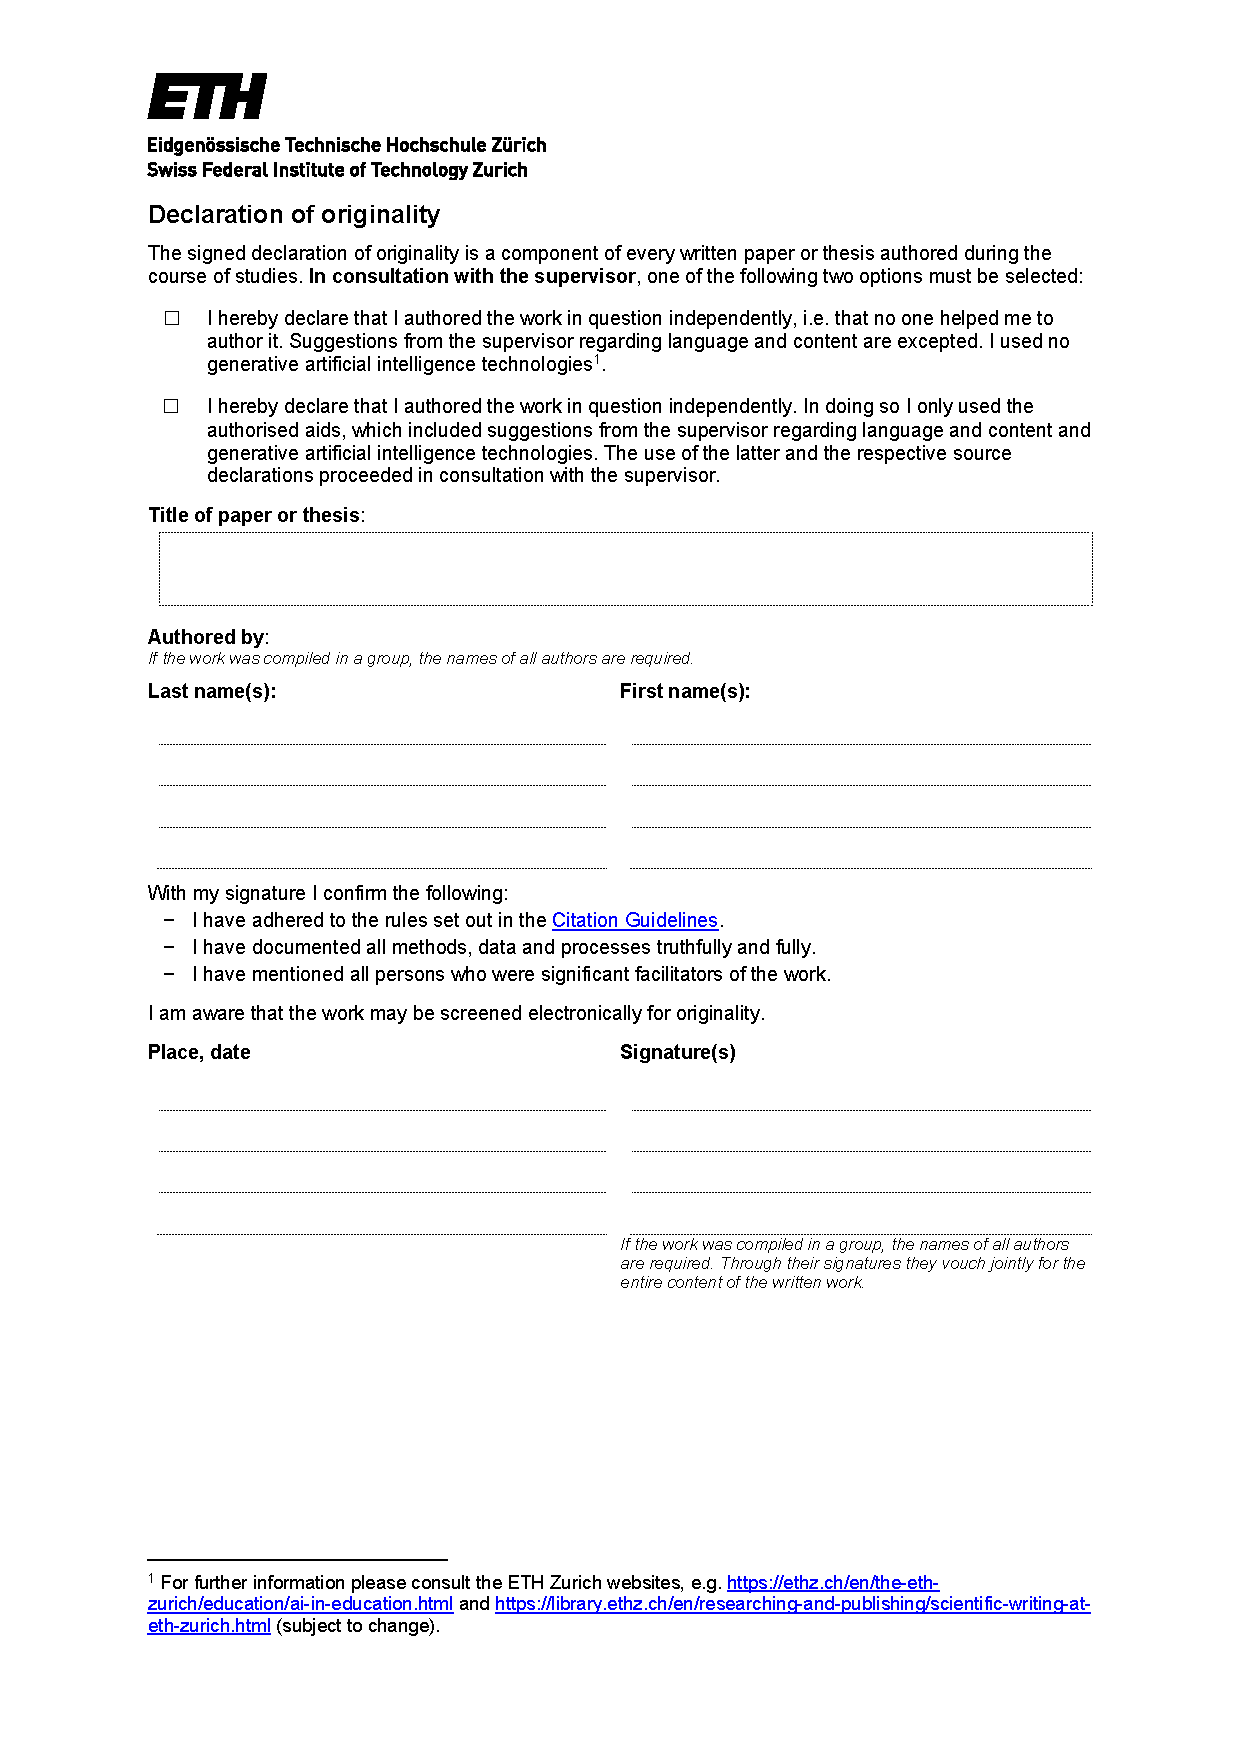
\includepdf[pages={-}]{declaration-originality.pdf}

\end{document}
